\chapter{Segment lotny}\label{ch:lotny}

\begin{sekcja}{Zestaw lotny}
Zestaw lotny (\emph{flight train}) to wszystko, co leci. Rysunek~\ref{fig:zestaw} pokazuje elementy i ich kolejność.

\begin{minipage}[c]{0.62\linewidth}\centering
\resizebox{\linewidth}{!}{\rysZestaw}
\end{minipage}\hfill
\begin{minipage}[c]{0.34\linewidth}\centering
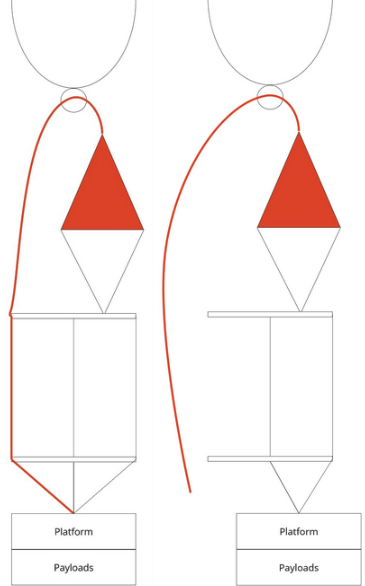
\includegraphics[width=0.8\linewidth]{rigging_cutter}
\end{minipage}
\captionof{figure}{Zestaw lotny z odcinaczem mechanicznym. Z prawej: schemat z misji z 26.05.2023 przed odcięciem i po odcięciu; czerwona linia -- linka odcinacza i zapas linki~\cite{pac2024}.}\label{fig:zestaw}
\end{sekcja}

\begin{sekcja}{Zestaw lotny w powietrzu}
\begin{minipage}[c]{0.4\linewidth}\centering
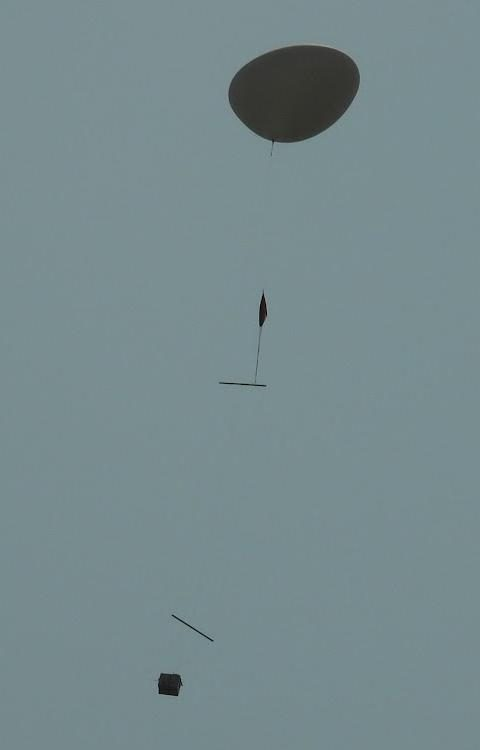
\includegraphics[width=\linewidth]{2023_zestaw_w_powietrzu_kadr}
\end{minipage}\hfill
\begin{minipage}[c]{0.55\linewidth}
Zestaw lotny Stardust NEXT krótko po starcie. Od góry widać:
\begin{enumerate}
  \item powłokę,
  \item spadochron (czerwony) na lince pod powłoką,
  \item poprzeczki z rurki na olinowaniu,
  \item zapas linki,
  \item gondolę.
\end{enumerate}
Linki są napięte, a elementy wiszą w jednej linii. Tak powinien wyglądać zestaw po prawidłowym starcie.
\end{minipage}
\captionof{figure}{Stardust NEXT w powietrzu (kadr ze zdjęcia z ziemi).}
\end{sekcja}

\begin{sekcja}{Powłoka}
\begin{itemize}
  \item Typ: lateksowa powłoka meteorologiczna (np. Hwoyee, Kaymont, Pawan). Dostawca w Polsce: \url{https://nearspace.pl/}.
  \item Wybierz rozmiar w kalkulatorze (rozdział~\ref{ch:planowanie}). Większa powłoka pęka wyżej, ale potrzebuje więcej gazu.
  \item Gaz nośny: hel. Wodór jest palny i wymaga dodatkowych środków bezpieczeństwa.
  \item Przechowuj powłokę w oryginalnym opakowaniu, w ciemnym i chłodnym miejscu.
  \item Dotykaj powłoki tylko w czystych rękawiczkach.
\end{itemize}
\end{sekcja}

\begin{sekcja}{Spadochron}
\begin{itemize}
  \item Dobierz spadochron do masy ładunku. Docelowa prędkość lądowania: około \SI{5}{m/s}.
  \item Spadochron wisi pod krętlikiem, nad gondolami. Jest stale otwarty -- nie ma mechanizmu wyrzutu.
  \item Kolor i średnicę spadochronu wpisz do zgłoszenia PAŻP.
\end{itemize}
\end{sekcja}

\begin{sekcja}{Olinowanie}
\textbf{Materiały:} taśma parciana, regulatory do taśmy (plastikowe albo metalowe), linka o średnicy około \SI{1}{mm} i wytrzymałości poniżej \SI{230}{N}, krętlik.

\textbf{Zasady:}
\begin{enumerate}
  \item Krętlik montuj bezpośrednio pod powłoką, na krótkiej pętli przywiązanej do szyjki. Krętlik zmniejsza skręcanie linek.
  \item Dodaj 10--15~m zapasu linki między spadochronem a gondolą. Zapas daje spadochronowi miejsce na otwarcie, gdy linki się skręcą.
  \item Gondole łącz taśmą z regulatorami. Regulatory pozwalają szybko wyrównać długości na stanowisku.
  \item Zabezpiecz każdy węzeł taśmą klejącą.
  \item Rozkładaj olinowanie na ziemi w linii, z wiatrem, bez pętli (rysunek~\ref{fig:pociag}).
\end{enumerate}

\foto[0.85\linewidth]{2023_zestaw_przed_startem}{Zestaw rozłożony przed startem: gondola na pierwszym planie, linka rozciągnięta w stronę stanowiska tankowania. Biała rurka pomaga rozłożyć linkę bez splątania.}\label{fig:pociag}
\end{sekcja}

\begin{sekcja}{Odcinacz mechaniczny -- zasada działania}
Odcinacz kończy lot na komendę albo automatycznie. Odcinacz oddziela gondole ze spadochronem od powłoki.

Odcinacz jest w gondoli platformy, nie pod balonem. Linka odcinacza biegnie od powłoki w dół do gondoli i jest zaczepiona o \textbf{zwalniacz serwomechaniczny} na pokrywie gondoli. Gdy serwo zwalnia linkę, gondole odłączają się od powłoki i opadają na spadochronie.

\textbf{Zalety:} cała elektronika jest w jednej gondoli. Odcinacz nie wymaga zasilania pod balonem.

\textbf{Wada:} obrót gondoli skręca linki. Skręcone linki mogą zablokować linkę odcinacza (misja z 26.05.2023).

\foto[0.55\linewidth]{2023_gondola_gora}{Pokrywa gondoli platformy: płyta montażowa (niebieska) ze zwalniaczem serwomechanicznym i zaczepioną linką, pasy z regulatorami, dwie anteny GPS.}
\end{sekcja}

\begin{sekcja}{Odcinacz mechaniczny -- wymagania}
\begin{itemize}
  \item Zwalniacz ładunku sterowany serwem (PWM, zasilanie 5--\SI{7.2}{V}, masa około \SI{76}{g}), np. zwalniacz zrzutu ładunku do dronów.
  \item Odcinacz działa na komendę z ziemi albo automatycznie: po czasie, po przekroczeniu wysokości, po wyjściu z dozwolonego obszaru, po długim locie poziomym (balon nie pękł).
  \item Komputer bezpieczeństwa (HABduino) steruje odcinaczem głównym. Komputer pokładowy (OBC) steruje \textbf{drugim, niezależnym odcinaczem innego typu}, np. z drutem oporowym (rozdział~\ref{ch:elektronika}).
  \item Testy: \SI{-40}{\degreeCelsius}, pełne obciążenie, skręcone linki (rozdział~\ref{ch:planowanie}).
  \item Na stanowisku sprawdź zwolnienie linki bez obciążenia, potem zaczep linkę i uzbrój odcinacz.
\end{itemize}

\renewcommand{\arraystretch}{1.3}
\small
\begin{tabularx}{\linewidth}{@{}P{32mm}P{38mm}L@{}}
\toprule
\textbf{Problem} & \textbf{Przyczyna} & \textbf{Środek zaradczy}\\\midrule
Linka odcinacza nie zwolniła się & Skręcone linki pod gondolą (brak krętlika na dole) & Zapas linki 10--15~m. Drugi krętlik nad gondolą. Prowadzenie linki odcinacza tak, aby skręt jej nie blokował.\\
Drut oporowy nie przeciął linki & Za krótki czas grzania & Testy w niskiej temperaturze i ciśnieniu. Dłuższy czas grzania. Bateria o większej wydajności prądowej.\\
\bottomrule
\end{tabularx}
\normalsize
\end{sekcja}

\begin{sekcja}{Gondola}
Gondola to pudełko styropianowe w rozmiarze typu eurobox (np. styrobox STX3-7, \SI{5}{l}). Pudełka są tanie, lekkie, izolują ciepło i chronią sprzęt przy lądowaniu. Mają standardowe wymiary, więc łatwo je łączyć ze sobą i z ładunkami zespołów badawczych.

\begin{center}\resizebox{0.9\linewidth}{!}{\rysGondola}\end{center}
\captionof{figure}{Przekrój gondoli: platforma (u góry) i ładunek badawczy (u dołu), spięte pasami.}\label{fig:gondola}
\end{sekcja}

\begin{sekcja}{Budowa gondoli platformy}
\begin{itemize}
  \item \textbf{Wkładka}: na dnie pudełka zamocuj płytę z lekkiego i wytrzymałego materiału (plexi, sklejka, włókno węglowe). Wszystkie elementy mocuj do wkładki: rzepem, śrubami, opaskami zaciskowymi. Uderzenie przy lądowaniu jest bardzo silne. Luźny element może zniszczyć resztę sprzętu, w tym karty pamięci -- a utrata danych to utrata całej misji.
  \item \textbf{Równowaga}: rozmieść elementy równomiernie. Środek masy musi leżeć w osi zawieszenia, aby gondola wisiała poziomo.
  \item \textbf{Płyta montażowa na pokrywie}: zwalniacz serwomechaniczny i mocowanie pasów.
  \item Gondola platformy zawiera tylko elektronikę platformy: tracker, OBC, odcinacz, lokalizatory, baterie.
  \item Anteny nadajników wyprowadź w dół. Antenę GPS umieść na górze, z widokiem na niebo, z dala od metalu.
  \item Opisz pudełko markerem: numer telefonu, „Projekt badawczy”, logo (rozdział~\ref{ch:prawo}).
\end{itemize}
\end{sekcja}

\begin{sekcja}{Gondola na zdjęciach}
\foto[0.8\linewidth]{2023_gondola_otwarta}{Gondola platformy otwarta: wkładka (czarna plexi) z elementami mocowanymi na rzep, śruby i opaski. Pokrywa z płytą montażową (niebieska), zwalniaczem i pasami.}
\dwafoto{2023_gondola_bok_anteny}{Anteny wyprowadzone w dół z boku gondoli.}
{2023_gondola_bok_termometr}{Platforma (u góry) i ładunek (u dołu) spięte pasami; czujnik temperatury na zewnątrz.}
\end{sekcja}

\begin{sekcja}{Anteny gondoli}
Antena typu dipol wymaga przeciwwagi. W powietrzu nie ma uziemienia -- przeciwwagą są przewody i elektronika w gondoli, co zmienia charakterystykę anteny.

Do rozważenia w kolejnych wersjach platformy:
\begin{itemize}
  \item metalowa płyta pod gondolą jako przeciwwaga i reflektor,
  \item antena ćwierćfalowa skierowana w dół, z luźnymi przewodami przeciwwagi (\emph{ground plane}),
  \item pomiar dopasowania anteny (SWR) w konfiguracji lotnej, w gondoli.
\end{itemize}
\end{sekcja}

\begin{sekcja}{Gondola ładunku badawczego}
\begin{itemize}
  \item Ładunek ma własne pudełko tego samego typu. Pudełka łączą się pasami.
  \item Ładunek ma własne zasilanie i własne oznakowanie.
  \item Ładunek przechodzi te same testy co platforma (rozdział~\ref{ch:planowanie}).
  \item Zespół badawczy podaje masę i częstotliwości radiowe (rozdział~\ref{ch:planowanie}).
\end{itemize}
\end{sekcja}
